% ===============================================================================
% = LaTeX Beamer Template des Arbeitsbereichs Sicherheit in verteilten Systemem
% = (c) 2012 Prof. Dr. Hannes Federrath, Uni Hamburg, Fachbereich Informatik
% = http://www.informatik.uni-hamburg.de/svs/
% ===============================================================================
%
\documentclass[t]{beamer}
% Option t              Place text of slides at the (vertical) top of the slides.
% Option handout        Ein PDF ohne Pausen und Overlayeffekte erzeugen.
% Option aspectratio=43 169 => 16:9, 1610 => 16:10, 43 => 4:3
\usepackage[utf8]{inputenc}
\usepackage[ngerman]{babel}
\usepackage{graphicx,xcolor}
\usepackage[T1]{fontenc} % 8-Bit-Zeichen; ermöglicht korrektes Kopieren von Umlauten aus dem pdf
\usepackage[scaled]{helvet}

\usepackage{beamerthemedefault}
\usepackage{listings}
\usepackage{comment}
\lstset{ %
  backgroundcolor=\color{white},   % choose the background color; you must add \usepackage{color} or \usepackage{xcolor}
  basicstyle=\footnotesize,        % the size of the fonts that are used for the code
  breakatwhitespace=false,         % sets if automatic breaks should only happen at whitespace
  breaklines=true,                 % sets automatic line breaking
  captionpos=b,                    % sets the caption-position to bottom
  commentstyle=\color{black},    % comment style
  deletekeywords={...},            % if you want to delete keywords from the given language
  escapeinside={\%*}{*)},          % if you want to add LaTeX within your code
  extendedchars=true,              % lets you use non-ASCII characters; for 8-bits encodings only, does not work with UTF-8
  frame=single,	                   % adds a frame around the code
  keepspaces=true,                 % keeps spaces in text, useful for keeping indentation of code (possibly needs columns=flexible)
  keywordstyle=\color{blue},       % keyword style
  language=Octave,                 % the language of the code
  otherkeywords={*,...},           % if you want to add more keywords to the set
  numbers=left,                    % where to put the line-numbers; possible values are (none, left, right)
  numbersep=5pt,                   % how far the line-numbers are from the code
  numberstyle=\tiny\color{gray}, % the style that is used for the line-numbers
  rulecolor=\color{black},         % if not set, the frame-color may be changed on line-breaks within not-black text (e.g. comments (green here))
  showspaces=false,                % show spaces everywhere adding particular underscores; it overrides 'showstringspaces'
  showstringspaces=false,          % underline spaces within strings only
  showtabs=false,                  % show tabs within strings adding particular underscores
  stepnumber=2,                    % the step between two line-numbers. If it's 1, each line will be numbered
  stringstyle=\color{mauve},     % string literal style
  tabsize=2,	                   % sets default tabsize to 2 spaces
  %title=\lstname                   % show the filename of files included with \lstinputlisting; also try caption instead of title
}
% Ränder definieren
\setbeamersize{text margin left=5ex, text margin right=5ex}

% Farbdefinitionen
\definecolor{svsgrau1}{RGB}{191,191,191} % Balken in Kopfzeile
\definecolor{svsgrau2}{RGB}{123,123,123} % Folienüberschriften
\definecolor{svsrot}{RGB}{255,0,0} % Bullets
\definecolor{svshellblau1}{RGB}{153,204,255} % Block Hintergrund
\definecolor{svshellblau2}{RGB}{24,113,248} % Anstrich Ebene 2
\definecolor{svsdunkelblau}{RGB}{38,82,128} % Text der Ebene 1

% Navigationsleiste ausblenden
\beamertemplatenavigationsymbolsempty

% Farben der Bullets der Ebenen
\setbeamercolor{itemize item}{fg=svsrot}
\setbeamercolor{itemize subitem}{fg=svshellblau2}
\setbeamercolor{enumerate item}{parent=itemize item}
\setbeamercolor{enumerate subitem}{parent=itemize subitem}

% Formen der Bullets der Ebenen
\setbeamertemplate{itemize item}[circle]
\setbeamertemplate{itemize subitem}{--}
\setbeamertemplate{itemize subsubitem}[circle]

% Farben der Texte
\setbeamercolor{title}{fg=black}
\setbeamercolor{structure}{fg=svsgrau2}
\setbeamercolor{section in toc}{fg=black}
\setbeamercolor{framesubtitle}{fg=svsdunkelblau}
\setbeamercolor{itemize/enumerate body}{fg=svsdunkelblau}
\setbeamercolor{itemize/enumerate subbody}{fg=black}
\setbeamercolor{itemize/enumerate subsubbody}{fg=black}

% Zeichensätze der Texte
\setbeamerfont{author}{size=\normalsize}
\setbeamerfont{institute}{size=\normalsize}
\setbeamerfont{date}{size=\normalsize}
\setbeamerfont{frametitle}{size=\large}
\setbeamerfont{framesubtitle}{size=\footnotesize\raggedleft}
\setbeamerfont{sections/subsections in toc}{size=\normalsize}
\setbeamerfont{itemize/enumerate body}{size=\normalsize}
\setbeamerfont{itemize/enumerate subbody}{size=\normalsize}
\setbeamerfont{itemize/enumerate subsubbody}{size=\normalsize}

% Definitionen für farbig hinterlegten Block
\setbeamertemplate{blocks}[rounded]
\setbeamercolor{block title}{fg=black,bg=svshellblau1}
\setbeamercolor{block body}{parent=normal text,use=block title,bg=block title.bg!25!bg}
\setbeamerfont{block title}{size=\normalsize}
\setbeamerfont{block body}{size=\normalsize}

% Definitionen für Agenda (FIXME: noch stärker an normale Listendefs. anpassen)
\setbeamertemplate{section in toc}[sections numbered]
\setbeamertemplate{subsection in toc}[square]

% Kopfzeile
\setbeamertemplate{headline}{
	
\includegraphics[height=8mm]{pic/UHH-Logo_2010_ohneText.png}%
	\color{svsgrau1}\rule{\paperwidth}{8mm}\newline
	\mbox{}\rule{1em}{0pt}\rule{0pt}{8ex}
	\dotfill\newline\vspace{-7.3ex}
}

% Fusszeile
\setbeamertemplate{footline}[text line]{
	\parbox[b]{50mm}{\insertframenumber\\[1ex]}
}

% Hintergrund Titelseite
\defbeamertemplate{background canvas}{titlepage}{%
	{\color{svsgrau1}\vrule width\paperwidth height0.7\paperheight}%
	{\color{white}\vrule width\paperwidth height0.3\paperheight}%
}

\def\therefore{
\leavevmode
\lower0.1ex\hbox{$\bullet$}
\kern-0.2em\raise0.7ex\hbox{$\bullet$}
\kern-0.2em\lower0.2ex\hbox{$\bullet$}
\thinspace}

% =============================
% = Ab hier Inhalte ändern...
% =============================

\title{IT-Sicherheit und Schutz vor Malware im Automobil}
\author[Beer, Grusche, Stock]{Arne Beer, Stefan Grusche, Joshua Stock}
% \institute[Uni Hamburg]{Universität Hamburg\\ Fachbereich Informatik}
\date{}

\begin{document}

\begingroup
	\setbeamertemplate{background canvas}[titlepage]
	\begin{frame}[plain]
		\vskip8mm
		
\includegraphics[width=2.2cm]{pic/svs_logo_hires-ohne-was.png}
		% \vskip-20mm % dies geht nur bei kurzen Vortragstiteln
		\titlepage
		\vspace{\fill}
		
\includegraphics[width=2.9cm]{pic/UHH-Logo_2010_Farbe_RGB_hires_nomargin.png}
		\vskip20pt
	\end{frame}
\endgroup

\begin{frame}{Gliederung}
	\tableofcontents
\end{frame}

\section{CAN-Bus}
\begin{frame}
    % Wir steigen nun relativ techni 787osch in das Thema ein.
	\frametitle{CAN-Bus: Was ist der CAN-Bus?}
	\begin{itemize}
  	    % Was sind ECU's, was sitzt am BUS
        \item Electron control Units (ECU's)
  	    % Ein Bus
		\item Zentrale Kommunikationsschnittstelle
        % Der CAN Bus
        \item Controller Area Network (CAN)
	\end{itemize}
\end{frame}

\begin{frame}
	\frametitle{CAN-Bus: Kommunikation am Can Bus}
	\begin{itemize}
        \item Alle Geräte kommunizieren gleichzeitig.
		\item Jedes Gerät sendet an jeden.
	\end{itemize}
    \begin{center}
        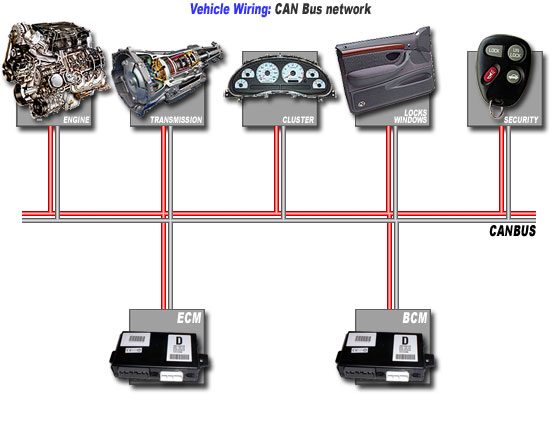
\includegraphics[width=0.8\textwidth]{pic/diag_canbus2.jpg} \ \
        % \caption[Can-Network]{Vereinfachtes CAN-Network}
        % \cite{Quellen}
    \end{center}
    % http://360.here.com/2014/12/19/can-bus-inside-your-car-and-why-does-here-care-about-it/
\end{frame}

\begin{frame}
	\frametitle{CAN-Bus: Unsicherheiten}
	\begin{itemize}
  	    % Carrier Sense Multiple Access/Collision Resolution (CSMA/CR)
        \item Kompletter Verkehr ist unverschlüsselt
		\item Keine Verschlüsselung
	\end{itemize}
    $\Rightarrow$ Sniffing
\end{frame}

\begin{frame}
	\frametitle{CAN-Bus: Messages}
    Ein CAN-Bus Paket:
    \newline
    \newline
    \newline
    \newline
    {\Large \centerline{\texttt{00 B4 08 00 00 00 00 3C 18 C0 FF}}}
    \vspace*{1cm}

    22 Hexadezimalstellen = 88 bit or 11 Byte
\end{frame}

\begin{frame}
	\frametitle{CAN-Bus: Messages}
    Ein CAN-Bus Paket:
    \newline
    \newline
    \newline
    \newline
    {\Large \centerline{\textbf{00 B4} \texttt{08 00 00 00 00 3C 18 C0 FF}}}
    \vspace*{1cm}

    Byte 1-2 Address
\end{frame}

\begin{frame}
	\frametitle{CAN-Bus: Messages}
    Ein CAN-Bus Paket:
    \newline
    \newline
    \newline
    \newline
    {\Large \centerline{\texttt{00 B4} \textbf{08} \texttt{00 00 00 00 3C 18 C0 FF}}}
    \vspace*{1cm}

    Byte 1-2 Address \\
    Byte 3 Payload length
\end{frame}

\begin{frame}
	\frametitle{CAN-Bus: Messages}
    Ein CAN-Bus Paket:
    \newline
    \newline
    \newline
    \newline
{\Large \centerline{\texttt{00 B4 08} \textbf{00 00 00 00 3C 18 C0} \texttt{FF}}}
    \vspace*{1cm}

    Byte 1-2 Address \\
    Byte 3 Payload length \\
    byte 4-10 Payload
\end{frame}

\begin{frame}
	\frametitle{CAN-Bus: Messages}
    Ein CAN-Bus Paket:
    \newline
    \newline
    \newline
    \newline
{\Large \centerline{\texttt{00 B4 08 00 00 00 00 3C 18 C0} \textbf{FF}}}
    \vspace*{1cm}

    Byte 1-2 Address \\
    Byte 3 Payload length \\
    Byte 4-10 Payload \\
    Byte 11 Checksum \\
    E.g.: $(IDH + IDL + Len + Sum(\text{Data}[0]\text{ – }\text{Data}[Len-2])) \& 0xFF $
\end{frame}


\begin{frame}
	\frametitle{CAN-Bus: Building your own packets}
    Wie einfach ist es eigene Pakete zu bauen?
    \newline
    \newline
    \newline
    \newline
    {\Large \centerline{\texttt{AA BB 00 00 CC DD 00 00}}}
    \newline
    \newline
    {\Large \centerline{\texttt{XX YY LL AA BB 00 00 CC DD 00 SS}}}
\end{frame}

\begin{frame}
	\frametitle{CAN-Bus: Building own packets}
    Tacho auf 100 km/h bei 2000 RPM!
    \newline
    \[\text{Speed} (mph) = 0.0065 \cdot (CC DD) - 67\]
    \[RPM = 0.25 \cdot (AA BB) - 24\]
\end{frame}

\begin{frame}
	\frametitle{CAN-Bus: Building own packets}
    Tacho auf 100 km/h bei 2000 RPM!
    \newline
    \[62.1371 = 0.0065 \cdot (CC DD) - 67\]
    \[2000 = 0.25 \cdot (AA BB) - 24\]
    \newline
    CC DD = 19846 = 4D86 \\
    AA BB = 8096 = 1FA0
    \newline
    \newline
    {\Large \centerline{\texttt{00 B4 08 1F A0 00 00 4D 86 00 CC}}}

\end{frame}


\section{Ausgewählte Angriffsvektoren} % erscheint in Agenda
\begin{frame}
	\frametitle{Angriffsvektoren: verwundbare Komponenten am CAN-Bus}
    \begin{center}
    	\begin{figure}
			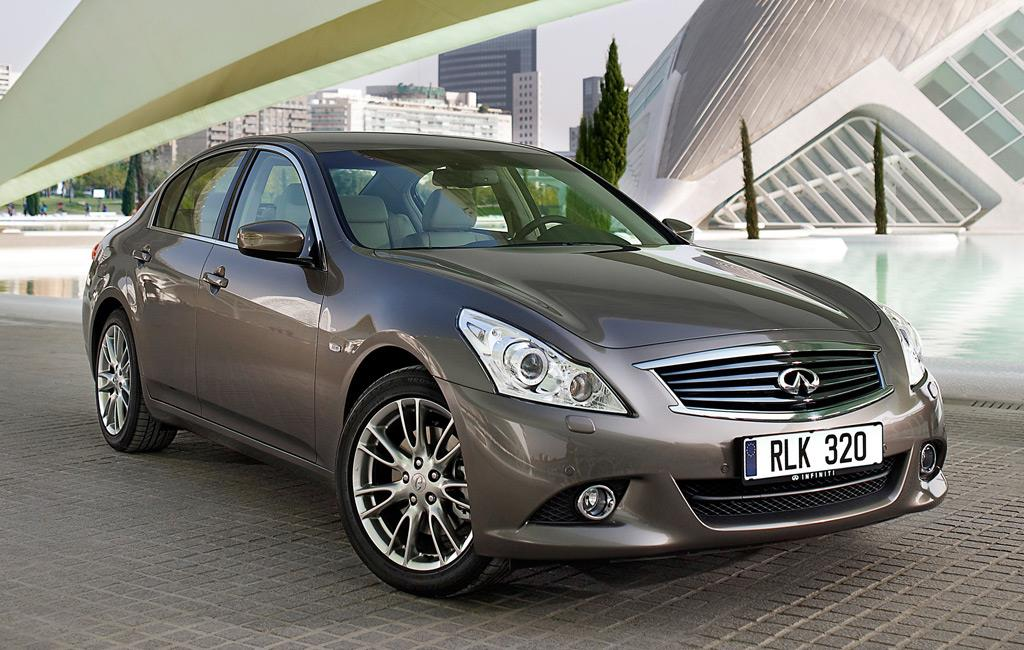
\includegraphics[width=0.3\textwidth]{pic/remote_attack_images-026.jpg} \ \
			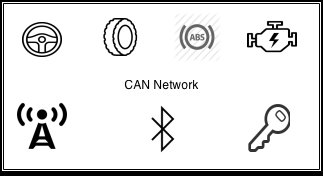
\includegraphics[width=0.3\textwidth]{pic/remote_attack_images-027.jpg}
      	  	\caption[2010 Infiniti G37 (Sedan)]{Sedan Infiniti (2010)\footnote{Quelle: http://images.thecarconnection.com/lrg/2010-infiniti-g37-sedan} und Komponenten im CAN-Netzwerk\footnote{Quelle: {[}MV14{]}}}
			% Lenkradkontrolle, Reifendrucksensoren, Bremssysteme, Motorkontroll-Einheit, AM/FM-Radio, Bluetooth, ferngesteuertes Öffnen bzw. Starten des Autos
			%Quellen für Bilder:
			% http://images.thecarconnection.com/lrg/2010-infiniti-g37-sedan_100234015_l.jpg
			% [MV14]
		\end{figure}
	\end{center}
	\begin{itemize}
		\item (zu) offene Schnittstellen
	    %z.B. Update über Internet ohne sichere Authentifizierung
  	    \item Unsaubere Implementierungen
  	    %z.B. muss Bluetooth-Modul Zugriff auf den Bus haben?
        \item Telematik-Modul bündelt ausgehende Verbindungen
        %Konnektivität des Autos
        % Telematic  Control  Units“:  Steuergeräte  für  Telematikdienste.  Sind  in  der  Regel  direkt  an  den  CAN-Bus angeschlossen und zeichnen sich häufig durch viele ausgehende Verbindungen aus (Bluetooth, Mobilfunk, GPS, etc.)
	\end{itemize}
\end{frame}

\subsection{Mobilfunk}
\begin{frame}
	\frametitle{Mobilfunk I}
    \begin{center}
        \begin{figure}
            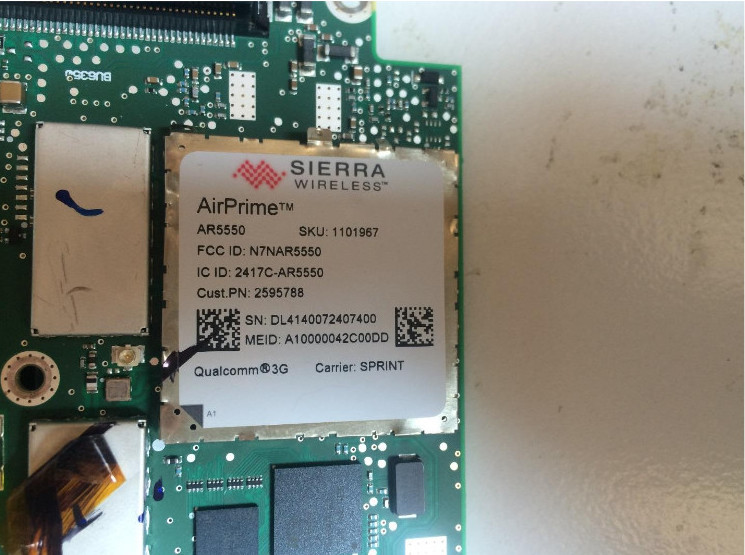
\includegraphics[width=0.3\textwidth]{pic/001_cellular.jpg}
            \caption[Mobilfunk]{Mobilfunk-Einheit im Jeep Cherokee, Quelle: [MV15]}
            %Sierra Wireless AirPrime AR5550 from a Harman Uconnect system
            %Quelle für Bild:
            % [MV15]
        \end{figure}
	\end{center}

    \begin{itemize}
		\item Funktionen:
        \begin{itemize}
        	\item Internetverbindung (3G) % z.B. für WLAN-Hotspot, Wetterbericht, Routenplaner
            % oder Hersteller: Ferndiagnose, Anti-Diebstahl-Tracking
            \item Mobilfunk % z.B. für Notrufe oder Hersteller-Updates
        \end{itemize}
    \end{itemize}
\end{frame}

\begin{frame}
	\frametitle{Mobilfunk II}
    \ \par
    \begin{itemize}
		\item Unbemerkte Anrufe an Telematik-Einheit sind möglich
        % 'stealth mode' für Hersteller (Diagnose), versteckt vor Nutzer
        % gibt Informationen über Auto preis
        \begin{itemize}
        	\item Modem übersetzt akustische Töne in Bits
            %  Airbiquity’s aqLink
            \item Verwundbarkeiten: Pufferüberlauf und Authentifizierung
            % 'zufällige' Challenge leicht zu durchschauen
            % Ungefähr jede 256. (falsche) Antwort wird als richtig erkannt
        \end{itemize}
	\end{itemize}

    \begin{itemize}
        \item Beispiel für Angriff:
        \begin{itemize}
        	\item Automatisiertes Anrufen bis Authentifizierung erfolgt
            \item Aufhebung der maximal erlaubten Anruflänge
            \item Download von zusätzlichem Code über 3G-Modem
            % Auch als in Hörer gespielte mp3 möglich
        \end{itemize}
        %Stephen  Checkoway,  Damon  McCoy,  Brian  Kantor, ... in Comprehensive experimental analyses of automotive attack surfaces
    \end{itemize}
\end{frame}

\subsection{WLAN} % erscheint in Gliederung
 \begin{frame}
	\frametitle{WLAN I}
    \begin{itemize}
		\item Funktion:
        \begin{itemize}
			\item Hotspot für Passagiere
		\end{itemize}
    \end{itemize}
    \begin{itemize}
		\item Hardware hat indirekten Zugriff auf CAN-Bus
	\end{itemize}
    \begin{itemize}
		\item Standard-Verschlüsselung: zufälliges WPA2-Passwort
		\begin{itemize}
			\item Zufallsalgorithmus basiert auf momentaner Systemzeit %in Sekunden
		\end{itemize}
	\end{itemize}
    \begin{itemize}
		\item Miller und Valasek extrahierten Algorithmus von OMAP-Chip in [MV15]
        % aus WiFiSvc Binärdatei
        % Open Multimedia Applications Platform
        % in Funktion WiFi.E:generateRandomAsciiKey()



	\end{itemize}
\end{frame}

 \begin{frame}
	\frametitle{WLAN II}
    \begin{itemize}
		\item Umwandlung Zufallszahl -> ASCII-Zeichen:
        \end{itemize}
\end{frame}

 \begin{frame}
	\frametitle{WLAN II}
    \begin{itemize}
		\item Umwandlung Zufallszahl -> ASCII-Zeichen:
    \end{itemize}
    \lstinputlisting[firstline=0, lastline=14, title=WLAN-Passwort-Generierung auf OMAP-Chip (1/2). Quelle {[}MV15{]}]{wlan-pwd.c}

\end{frame}

 \begin{frame}
	\frametitle{WLAN III}
    \lstinputlisting[firstline=15, title=WLAN-Passwort-Generierung auf OMAP-Chip (2/2). Quelle {[}MV15{]}]{wlan-pwd.c}

\end{frame}

\subsection{Bluetooth} % erscheint in Gliederung

\begin{frame}
	\frametitle{Bluetooth}
    \begin{itemize}
		\item
    \end{itemize}
\end{frame}

\section{Beispiel Jeep-Hack}
\begin{frame}
	\frametitle{Hack des 2014er Jeep Cherokees}
	\begin{figure}
        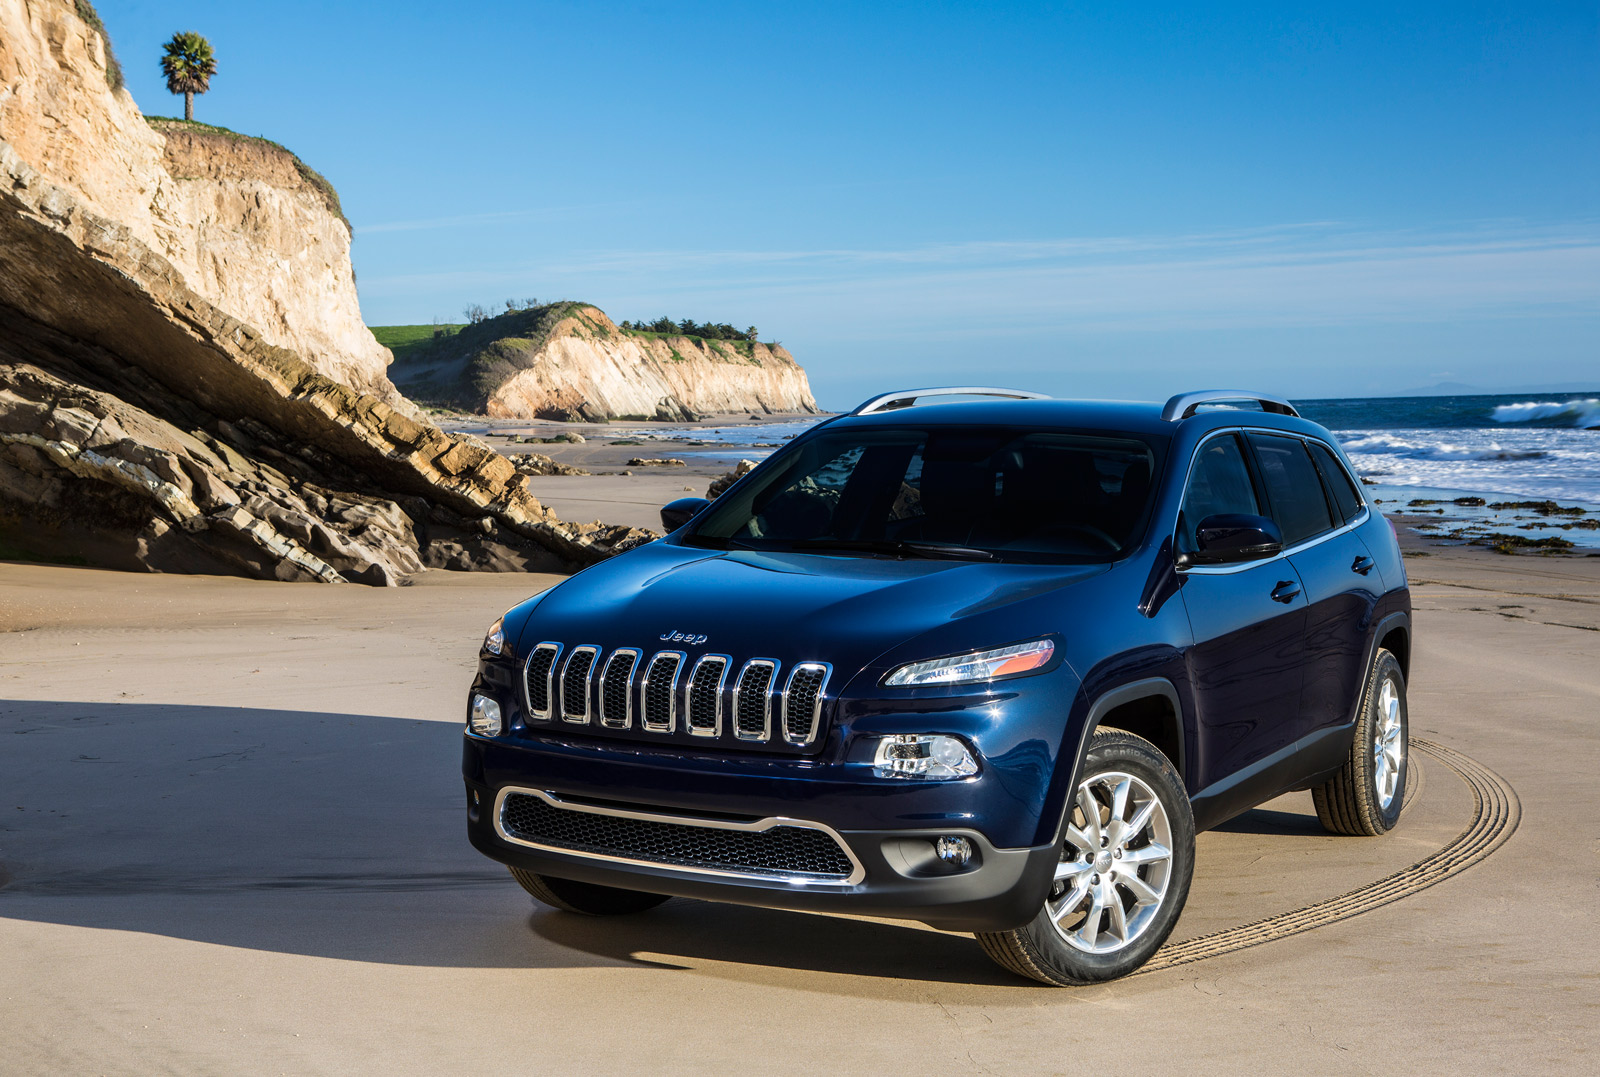
\includegraphics[width=0.6\textwidth]{pic/2014-jeep-cherokee-1.jpg} %http://www.blogcdn.com/www.autoblog.com/media/2013/02/2014-jeep-cherokee-1.jpg
        \caption{Ziel des Angriffs: 2014 Jeep Cherokee}
    \end{figure}
    \begin{itemize}
		\item veröffentlicht im Juli 2015
        \item durchgeführt von Charlie Miller und Chris Valasek
	\end{itemize}
\end{frame}

\begin{frame}
	\frametitle{Jeep Cherokee: CAN-Netzwerk}
    \begin{figure}
		\includegraphics[width=0.45\textwidth]{pic/jeep_cannets.png}
        \caption{Übersicht über CAN-Netze}
	\end{figure}
    \begin{itemize}
		\item zwei CAN-Netzwerke
        \item Funkmodul in beiden Netzen
	\end{itemize}
\end{frame}

\begin{frame}
    \frametitle{Fahrassistenzsysteme des Jeeps}
    \begin{figure}
        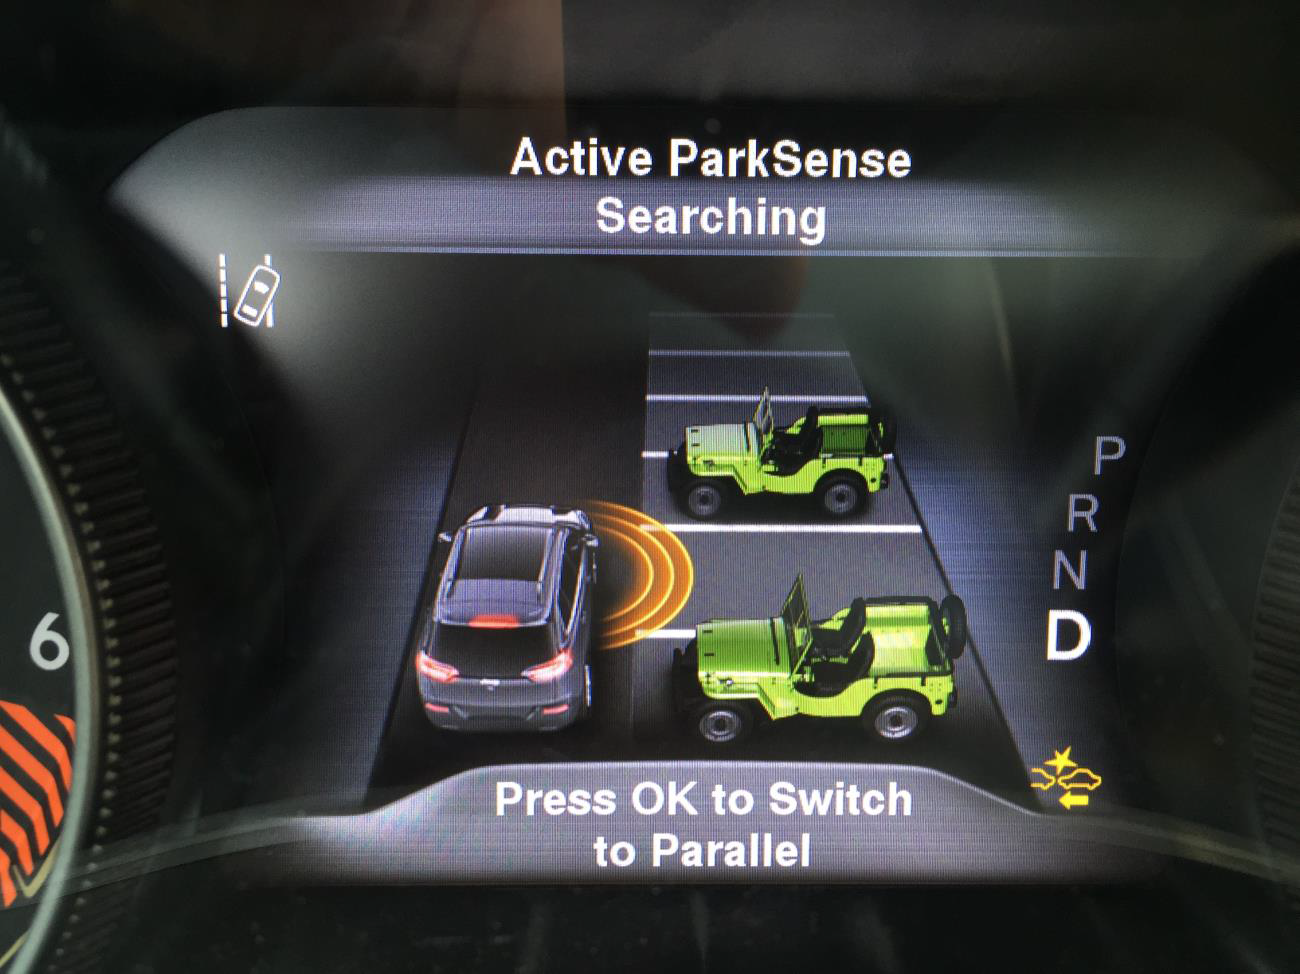
\includegraphics[width=0.48\textwidth]{pic/jeep_parkass.png}
        \caption{}
    \end{figure}
    \begin{itemize}
        \item adaptiver Tempomat
        \item Kollisionswarnsystem
        \item Spurhalteassistent
        \item Parkassistent
    \end{itemize}
\end{frame}

\begin{frame}
	\frametitle{Angriffsvektoren des Jeeps}
    \begin{itemize}
		\item Bluetooth
        \begin{itemize}
			\item herkömmliche Angriffe möglich
		\end{itemize}

    	\item Radio
        	\begin{itemize}
				\item vermutlich keine Code-Ausführung zu erreichen
			\end{itemize}

        \item WLAN
        	\begin{itemize}
				\item herkömmliche Angriffe / Schwäche bei Standardpasswörtern
			\end{itemize}

        \item Mobilfunk / Mobiles Internet
       		\begin{itemize}
				\item Möglicher Zugriff über große Distanzen
			\end{itemize}
	\end{itemize}
    $\Rightarrow$ UConnect-Mediensystem verbindet sämtliche Faktoren
\end{frame}

\begin{frame}
	\frametitle{UConnect-System von Harman Kardon}
    \begin{itemize}
    	\item Radio, WLAN, Navigation, Apps, Freisprechanlage...
        \item Funktionalität auf einem TI-Chip
        \item Kommuniziert mit CAN-Netzen über separaten Controller
        \item Für Vielzahl an Modellen verfügbar
    \end{itemize}
\end{frame}

\begin{frame}
	\frametitle{UConnect-System von Harman Kardon}
    \begin{itemize}
    	\item im WLAN-Netz diverse offene Ports identifizierbar
    	\item IPC-Dienst D-Bus an Port 6667
    	\item D-Bus ohne Authentifizierung nutzbar:
   	\end{itemize}
    \begin{figure}
    \includegraphics[width=0.7\textwidth]{pic/dbusauth.png}
    \caption{Anonymer Zugriff auf D-Bus}
    \end{figure}
\end{frame}

\begin{frame}
	\frametitle{D-Bus-Exploit}
	\begin{itemize}
    	\item Debug-Tools u. Bibliotheken zeigen nutzbare Dienste
        \begin{itemize}
        \item z.B. \texttt{NavTrailService} enthält unsichere Methoden
        \item \texttt{execute} führt beliebige Shell-Befehle aus
        \end{itemize}
        \item Simple Lua-Skripte beeinflussen versch. Systeme:
    \end{itemize}
    \includegraphics[width=1\textwidth]{pic/setVolume.png}
    \begin{itemize}
    \item Zugriff auf
    \begin{itemize}
    \item GPS-Daten
    \item Lautstärke / Bass und Deaktivieren der Drehregler
    \item Lüftung
    \item Bildschirm
    \item ...
    \end{itemize}
    \end{itemize}
\end{frame}

\begin{frame}
	\frametitle{Zugriff über Mobilfunk}
\end{frame}
\section{Fazit}
\begin{frame}
	\frametitle{Fazit}
	\begin{itemize}
		\item Alles super
        %to be continued
	\end{itemize}
\end{frame}


\end{document}
